%!TEX program = xelatex
\let\stop\empty

\documentclass[12pt,a4paper,fontset=none]{exam-zh}
% ==========================
% 卷面变量设置（只需改这里）
% ==========================
\newcommand{\paperlevel}{高中一}
\newcommand{\papersubject}{数学 试卷二}
\newcommand{\schoolname}{金宝培元独立中学}
\newcommand{\examname}{年终考}
\newcommand{\classinfo}{S1(Y / H)}
\newcommand{\examdate}{3-11-2026}
\newcommand{\examtime}{12:10-12:55}
\newcommand{\questiontotal}{12}
\newcommand{\paperpercentage}{30\%}
\newcommand{\setterteacher}{蔡杰庆师}
\newcommand{\reviewteacher}{王萌师}
\newcommand{\auditteacher}{雷泳健师}



\usepackage{xeCJK}
\setCJKmainfont{Noto Serif CJK SC}
\newCJKfontfamily\heiti{Noto Serif CJK SC}
\newCJKfontfamily\kaishu{Noto Serif CJK SC}
\usepackage{geometry}
\usepackage{array}
\usepackage{tikz}
\usetikzlibrary{calc,angles,quotes}
\usepackage{amsmath}
\usepackage{wrapfig}
\usepackage{adjustbox}
\usepackage{enumitem}
\usepackage{fancyhdr}
\usepackage{scalerel}
\providecommand{\wideparen}[1]{\overset{\frown}{#1}}
\def\mcirc{\mathbin{\scalerel*{\circ}{j}}}
\def\msquare{\mathord{\scalerel*{\Box}{gX}}}
\geometry{margin=2cm}

% \AtBeginDocument{\zihao{4}}
% ----------- 调整 exam -----------


% --- 全局样式定义 ---
% 定义选择题环境：题号 1. 2.，选项 A. B. C. D. 粗体，且保留 1.5em 间距
\examsetup{
    page = {
    size = a4paper,           % 设定纸张大小 [4]
    foot-content = { - ; - }  % 页脚显示为 -1-, -2- 格式 [3]
  },
    choices = {
    label-pos = top-left,
    column-sep = 1em,
    label-pos = auto,
    label-sep = 0.5em,
    max-columns = 4
    },
  question = {
    top-sep    = 1em, % 调整题目上方的垂直距离（默认值为 .5em plus .5em minus .2em）
    bottom-sep = 1em  % 调整题目下方的垂直距离（默认值为 .5em plus .5em minus .2em）
  },
    paren = {
    show-paren = false  % 设置为 false 则不显示括号 [3, 4]
  },
    choices = {
    label = \textbf{\Alph*}
  }, 
    solution = {
    show-solution = show-move, % 答案自动移动到卷末
    label-content = {参考答案},  % 答案区的标题文字
    show-qed = true            % 在解答末尾显示结束符号 ◻ 
  }
}



\makeatletter
\newcounter{answerkeyquestion}
\let\answerkeytotal\questiontotal
\let\originalparen\paren
\newcommand{\answerkeyitems}{}
\newcommand{\addanswerkeyitem}[2]{%
  \pgfmathtruncatemacro{\row}{ifthenelse(#1<=\cols,0,1)}%
  \pgfmathtruncatemacro{\col}{mod(#1-1,\cols)}%
  \pgfmathsetlengthmacro{\x}{\col*\boxw}%
  \pgfmathsetlengthmacro{\y}{-\row*\boxh}%
  \draw (\x,\y) rectangle ++(\boxw,\boxh);%
  \node[anchor=north west] at (\x+\offset,\y+\boxh-\offset) {\textbf{#1.}};%
  \node at (\x+0.6*\boxw,\y+0.45*\boxh) {\Large\textbf{#2}};%
}
\renewcommand{\paren}[1][]{%
  \originalparen[#1]%
  \edef\answerkeytemp{#1}%
  \ifx\answerkeytemp\@empty\else
    \stepcounter{answerkeyquestion}%
    \begingroup
      \edef\x{\endgroup
        \noexpand\g@addto@macro\noexpand\answerkeyitems{\noexpand\addanswerkeyitem{\theanswerkeyquestion}{#1}}}%
    \x
  \fi
}
\makeatother

\newcommand{\makeexamheader}{%
% ==========================
% 三栏标题区
% ==========================
\noindent
\begin{tabular*}{\textwidth}{@{\extracolsep{\fill}} p{0.3\textwidth} p{0.35\textwidth} p{0.3\textwidth}}

\raggedright
\textbf{\paperlevel}\\[0.2em]
\textbf{}{\papersubject}\\[0.4em]
姓名：\underline{\hspace{3cm}} &

\centering
\textbf{\schoolname}\\[0.2em]
\textbf{\examname}\\[0.4em]
班级：\classinfo&

\raggedright
日期：\examdate\\[0.2em]
时间：\examtime\\[0.4em]
得分：\underline{\hspace{2.5cm}} \\

\end{tabular*}

\begin{flushleft}
考生须知： 
选出正确的答案，用蓝或黑色的原子笔将答案的相应选项字母填入本页特备作答栏。
\end{flushleft}

% =========================
% 答题栏
% =========================
\begin{flushleft}
\textbf{特备答题栏:}
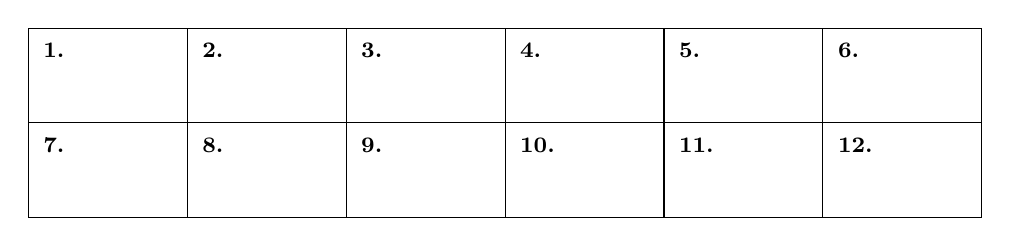
\begin{tikzpicture}
  % ---- 12题：6×2 ----
  \pgfmathtruncatemacro{\cols}{6}
  \pgfmathsetlengthmacro{\boxw}{(\linewidth-0.4pt)/\cols}
  \pgfmathsetlengthmacro{\boxh}{1.2cm}
  \pgfmathsetlengthmacro{\offset}{0.15cm}

  \foreach \num in {1,...,\answerkeytotal} {
    \pgfmathtruncatemacro{\row}{ifthenelse(\num<=\cols,0,1)}
    \pgfmathtruncatemacro{\col}{mod(\num-1,\cols)}
    \pgfmathsetlengthmacro{\x}{\col*\boxw}
    \pgfmathsetlengthmacro{\y}{-\row*\boxh}
    \draw (\x,\y) rectangle ++(\boxw,\boxh);
    \node[anchor=north west, font=\footnotesize, inner sep=1pt] at (\x+\offset,\y+\boxh-\offset) {\textbf{\num.}};
  }
\end{tikzpicture}

\end{flushleft}
}


\begin{document}
\makeexamheader
%region 范围：第 9 章 任意角的三角函数 | 考点：9.1 象限角、三角函数定义、相伴锐角 | 难度：易
\begin{question}
    如图，角 $\theta$ 的终边经过点 $P$，$\alpha$ 为 $\theta$ 的相伴锐角，则 $\cos\alpha=$ \paren[C]
    \begin{center}
        \begin{tikzpicture}[scale=0.8, >=stealth]
            % 坐标轴
            \draw[->] (-4.5,0) -- (3,0) node[right] {$x$};
            \draw[->] (0,-0.8) -- (0,5.5) node[above] {$y$};
            \node[below left] at (0,0) {$O$};
            % 终边与点 P
            \coordinate (P) at (-3,4);
            \draw[thick] (0,0) -- (P);
            \fill (P) circle (1.5pt) node[above left] {$P(-3,4)$};
            % 垂线与直角记号
            \draw[dashed] (P) -- (-3,0);
            \draw (-3,0) ++(0,0.3) -| ++(0.3,-0.3);
            % 角 theta：从 x 轴非负半轴逆时针到 OP
            \draw[->] (0.7,0) arc (0:126.87:0.7);
            \node at (60:1.05) {$\theta$};
            % 相伴锐角 alpha：OP 与 x 轴负半轴的夹角
            \draw[->] (126.87:1.2) arc (126.87:180:1.2);
            \node at (153:1.6) {$\alpha$};
        \end{tikzpicture}
    \end{center}
    \begin{choices}
        \item $-\dfrac{4}{5}$
        \item $-\dfrac{3}{5}$
        \item $\dfrac{3}{5}$
        \item $\dfrac{4}{5}$
    \end{choices}
\end{question}

\begin{solution}
    由图求 $\theta$ 的相伴锐角 $\alpha$ 的余弦值。 \\
    $\alpha$ 是 $OP$ 与 $x$ 轴所成的锐角，在 Rt$\triangle$ 中用邻边比斜边求 $\cos\alpha$。 \\
    设 $r=|OP|$，则
    \begin{align*}
        r &= \sqrt{(-3)^2+4^2} = 5 \\
        \cos\alpha &= \frac{|-3|}{r} = \frac{3}{5}
    \end{align*}
    故选 C。
\end{solution}
%endregion

%region 范围：第 9 章 任意角的三角函数 | 考点：9.1/9.2 特殊角函数值、符号判断、诱导公式求值 | 难度：易
\begin{question}
    $\sin 840^{\circ}+\cos(-300^{\circ})=$ \paren[D]
    \begin{choices}
        \item $-\dfrac{\sqrt{3}+1}{2}$
        \item $\dfrac{1-\sqrt{3}}{2}$
        \item $\dfrac{\sqrt{3}-1}{2}$
        \item $\dfrac{\sqrt{3}+1}{2}$
    \end{choices}
\end{question}

\begin{solution}
    求 $\sin 840^{\circ}+\cos(-300^{\circ})$ 的值。 \\
    先用 $360^{\circ}$ 的周期和 $-\theta$ 的诱导公式化为 $0^{\circ}\sim 90^{\circ}$ 的特殊角，再代入特殊角函数值。 \\
    \begin{align*}
        \sin 840^{\circ} &= \sin(2\times 360^{\circ}+120^{\circ}) = \sin 120^{\circ} = \sin(180^{\circ}-60^{\circ}) = \sin 60^{\circ} = \frac{\sqrt{3}}{2} \\
        \cos(-300^{\circ}) &= \cos 300^{\circ} = \cos(360^{\circ}-60^{\circ}) = \cos 60^{\circ} = \frac{1}{2} \\
        \sin 840^{\circ}+\cos(-300^{\circ}) &= \frac{\sqrt{3}}{2}+\frac{1}{2} = \frac{\sqrt{3}+1}{2}
    \end{align*}
    故选 D。
\end{solution}
%endregion

%region 范围：第 9 章 任意角的三角函数 | 考点：9.3 图像的值域 | 难度：易
\begin{question}
    函数 $f(x)=3\cos\left(2x+\dfrac{\pi}{3}\right)-1$ 的值域为 \paren[A]？
    \begin{choices}
        \item $[-4,\,2]$
        \item $[-3,\,3]$
        \item $[-2,\,0]$
        \item $[-2,\,4]$
    \end{choices}
\end{question}

\begin{solution}
    求函数 $f(x)=3\cos\left(2x+\frac{\pi}{3}\right)-1$ 的值域。 \\
    由 $-1\le\cos\left(2x+\frac{\pi}{3}\right)\le 1$ 逐步变形求值域。 \\
    \begin{align*}
        -1 \le \cos\left(2x+\frac{\pi}{3}\right) \le 1 &\Rightarrow -3 \le 3\cos\left(2x+\frac{\pi}{3}\right) \le 3 \\
        &\Rightarrow -4 \le 3\cos\left(2x+\frac{\pi}{3}\right)-1 \le 2
    \end{align*}
    故值域为 $[-4,\,2]$，故选 A。
\end{solution}
%endregion

\newpage

%region 范围：第 9 章 任意角的三角函数 | 考点：9.2 同角三角函数的基本关系（弦化切） | 难度：易
\begin{question}
    已知 $\tan\theta=-7$，则 $\dfrac{3\sin\theta+2\cos\theta}{2\sin\theta+3\cos\theta}$ 的值为 \paren[D]？
    \begin{choices}
        \item $-\dfrac{19}{11}$
        \item $\dfrac{11}{19}$
        \item $\dfrac{23}{17}$
        \item $\dfrac{19}{11}$
    \end{choices}
\end{question}

\begin{solution}
    已知 $\tan\theta=-7$，求 $\dfrac{3\sin\theta+2\cos\theta}{2\sin\theta+3\cos\theta}$ 的值。 \\
    因 $\tan\theta$ 有意义，故 $\cos\theta\neq0$，分子分母同除以 $\cos\theta$，化为关于 $\tan\theta$ 的式子。 \\
    \begin{align*}
        \frac{3\sin\theta+2\cos\theta}{2\sin\theta+3\cos\theta} &= \frac{3\tan\theta+2}{2\tan\theta+3} \\
        &= \frac{3\times(-7)+2}{2\times(-7)+3} \\
        &= \frac{-19}{-11} = \frac{19}{11}
    \end{align*}
    故选 D。
\end{solution}
%endregion

%region 范围：第 11 章 三角恒等式与三角方程式 | 考点：11.1 同角基本关系（知一求其余） | 难度：易
\begin{question}
    已知 $\cos\alpha=-\dfrac{5}{13}$，且 $\alpha$ 为第三象限角，则 $\tan\alpha=$ \paren[D]
    \begin{choices}
        \item $-\dfrac{12}{5}$
        \item $-\dfrac{5}{12}$
        \item $\dfrac{5}{12}$
        \item $\dfrac{12}{5}$
    \end{choices}
\end{question}

\begin{solution}
    已知 $\cos\alpha=-\frac{5}{13}$ 且 $\alpha$ 在第三象限，求 $\tan\alpha$。 \\
    先由平方关系求 $\sin\alpha$（第三象限 $\sin\alpha<0$），再由商的关系得 $\tan\alpha$。 \\
    \begin{align*}
        \sin^2\alpha &= 1-\cos^2\alpha = 1-\frac{25}{169} = \frac{144}{169} \\
        \sin\alpha &= -\frac{12}{13} \\
        \tan\alpha &= \frac{\sin\alpha}{\cos\alpha} = \left(-\frac{12}{13}\right)\times\left(-\frac{13}{5}\right) = \frac{12}{5}
    \end{align*}
    故选 D。
\end{solution}
%endregion

%region 范围：第 10 章 三角学的应用 | 考点：10.2 余弦定律（已知三边求角） | 难度：易
\begin{question}
    若三角形的三边长分别为 $4\ \mathrm{cm}$、$5\ \mathrm{cm}$ 及 $6\ \mathrm{cm}$，则它的最小内角约为 \paren[A]？
    \begin{choices}
        \item $41.4^{\circ}$
        \item $48.6^{\circ}$
        \item $55.8^{\circ}$
        \item $82.8^{\circ}$
    \end{choices}
\end{question}

\begin{solution}
    求三边为 $4,5,6$ 的三角形的最小内角。 \\
    最小边所对的角最小，故设边长 $4$ 所对的角为 $\alpha$，用余弦定律求 $\cos\alpha$。 \\
    \begin{align*}
        \cos\alpha &= \frac{5^2+6^2-4^2}{2\times5\times6} = \frac{45}{60} = \frac{3}{4} \\
        \alpha &= \cos^{-1}\frac{3}{4} \approx 41.4^{\circ}
    \end{align*}
    故选 A。
\end{solution}
%endregion

%region 范围：第 11 章 三角恒等式 | 考点：11.2 两角和差公式求值 | 难度：易
\begin{question}
    $\sin 75^\circ$ 的值为 \paren[C]？
    \begin{choices}
        \item $\dfrac{\sqrt{6}-\sqrt{2}}{4}$
        \item $\dfrac{\sqrt{6}}{4}$
        \item $\dfrac{\sqrt{6}+\sqrt{2}}{4}$
        \item $\dfrac{\sqrt{3}+1}{2}$
    \end{choices}
\end{question}

\begin{solution}
    求 $\sin 75^\circ$ 的值。 \\
    将 $75^\circ$ 拆成 $45^\circ+30^\circ$，用两角和的正弦公式 $\sin(\alpha+\beta)=\sin\alpha\cos\beta+\cos\alpha\sin\beta$。 \\
    \begin{align*}
        \sin 75^\circ&=\sin(45^\circ+30^\circ) \\
        &=\sin 45^\circ\cos 30^\circ+\cos 45^\circ\sin 30^\circ \\
        &=\frac{\sqrt{2}}{2}\times\frac{\sqrt{3}}{2}+\frac{\sqrt{2}}{2}\times\frac{1}{2} \\
        &=\frac{\sqrt{6}+\sqrt{2}}{4}
    \end{align*}
    故选 C。
\end{solution}
%endregion

%region 范围：第 10 章 三角学的应用 | 考点：10.1+10.2 正弦定律与三角形面积 | 难度：易
\begin{question}
    如图，在 $\triangle ABC$ 中，$\angle A=60^{\circ}$，$\angle B=45^{\circ}$，$BC=2\sqrt{6}$，则 $\triangle ABC$ 的面积为 \paren[C]？
    \begin{center}
        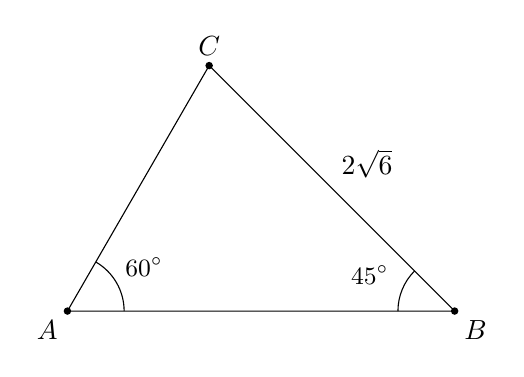
\begin{tikzpicture}[scale=0.9]
            \coordinate (A) at (0,0);
            \coordinate (B) at (5.464,0);
            \coordinate (C) at (2,3.464);
            \draw (A)--(B)--(C)--cycle;
            % 角的记号
            \draw (0.8,0) arc (0:60:0.8);
            \node at (30:1.25) {\small $60^\circ$};
            \draw ($(B)+(135:0.8)$) arc (135:180:0.8);
            \node at ($(B)+(157:1.3)$) {\small $45^\circ$};
            % 点与标注
            \fill (A) circle (1.5pt) node[below left]{$A$};
            \fill (B) circle (1.5pt) node[below right]{$B$};
            \fill (C) circle (1.5pt) node[above]{$C$};
            \path (B)--(C) node[midway,above right]{$2\sqrt{6}$};
        \end{tikzpicture}
    \end{center}
    \begin{choices}
        \item $3+\sqrt{3}$
        \item $4\sqrt{3}$
        \item $6+2\sqrt{3}$
        \item $12+4\sqrt{3}$
    \end{choices}
\end{question}

\begin{solution}
    求 $\triangle ABC$ 的面积。 \\
    先由正弦定律求 $AC$，再求 $\angle C$，用 $S=\frac{1}{2}\,BC\cdot AC\sin C$ 求面积。 \\
    设 $BC=a,\ AC=b$，则
    \begin{align*}
        \frac{b}{\sin B} &= \frac{a}{\sin A} \\
        b &= \frac{2\sqrt{6}\times\frac{\sqrt{2}}{2}}{\frac{\sqrt{3}}{2}} = 4 \\
        \angle C &= 180^{\circ}-60^{\circ}-45^{\circ} = 75^{\circ} \\
        \sin75^{\circ} &= \sin(45^{\circ}+30^{\circ}) = \frac{\sqrt{6}+\sqrt{2}}{4} \\
        S &= \frac{1}{2}\,ab\sin C = \frac{1}{2}\times2\sqrt{6}\times4\times\frac{\sqrt{6}+\sqrt{2}}{4} \\
        &= \sqrt{6}\,(\sqrt{6}+\sqrt{2}) = 6+2\sqrt{3}
    \end{align*}
    故选 C。
\end{solution}
%endregion

%region 范围：第 11 章 三角恒等式 | 考点：11.3 二倍角公式化简与求值 | 难度：中
\begin{question}
    已知 $\sin\alpha=\dfrac{3}{5}$，且 $\alpha\in\left(\dfrac{\pi}{2},\,\pi\right)$，则 $\tan2\alpha=$ \paren[A]
    \begin{choices}
        \item $-\dfrac{24}{7}$
        \item $-\dfrac{24}{25}$
        \item $\dfrac{7}{25}$
        \item $\dfrac{24}{7}$
    \end{choices}
\end{question}

\begin{solution}
    已知 $\sin\alpha=\frac{3}{5}$，$\alpha$ 为第二象限角，求 $\tan2\alpha$。 \\
    先由平方关系求 $\cos\alpha$（注意符号），再求 $\sin2\alpha$、$\cos2\alpha$，最后相除。 \\
    \begin{align*}
        \cos\alpha&=-\sqrt{1-\sin^2\alpha}=-\frac{4}{5} \\
        \sin2\alpha&=2\sin\alpha\cos\alpha=2\times\frac{3}{5}\times\left(-\frac{4}{5}\right)=-\frac{24}{25} \\
        \cos2\alpha&=1-2\sin^2\alpha=1-\frac{18}{25}=\frac{7}{25} \\
        \tan2\alpha&=\sin2\alpha\div\cos2\alpha=-\frac{24}{25}\times\frac{25}{7}=-\frac{24}{7}
    \end{align*}
    故选 A。
\end{solution}
%endregion

\newpage

%region 范围：第 10 章 解三角形 | 考点：10.4 方位角（读图与基本计算） | 难度：中
\begin{question}
    如图，一艘船从 $A$ 处出发向正东航行，在 $A$ 处测得灯塔 $C$ 在北偏东 $15^\circ$ 方向；航行 $20$ 海里到达 $B$ 处，测得灯塔 $C$ 在北偏西 $30^\circ$ 方向，则 $A$ 处到灯塔 $C$ 的距离为几海里\paren[D]？
    \begin{center}
        \begin{tikzpicture}
            \coordinate (A) at (0,0);
            \coordinate (B) at (5,0);
            \coordinate (C) at (75:6.12);
            \coordinate (NA) at (0,3.2);
            \coordinate (NB) at (5,3.2);
            \draw (A)--(B)--(C)--cycle;
            \draw[dashed,->] (A)--(NA);
            \draw[dashed,->] (B)--(NB);
            \pic[draw,"$15^\circ$",angle radius=12mm,angle eccentricity=1.5]{angle=C--A--NA};
            \pic[draw,"$30^\circ$",angle radius=12mm,angle eccentricity=1.5]{angle=NB--B--C};
            \fill (A) circle (1.5pt) node[below left]{$A$};
            \fill (B) circle (1.5pt) node[below right]{$B$};
            \fill (C) circle (1.5pt) node[above]{$C$};
            \node[above] at (NA){北};
            \node[above] at (NB){北};
            \node[below] at ($(A)!0.5!(B)$){$20$ 海里};
        \end{tikzpicture}
    \end{center}
    \begin{choices}
        \item $10\sqrt{2}$
        \item $\dfrac{20\sqrt{6}}{3}$
        \item $10\sqrt{3}$
        \item $10\sqrt{6}$
    \end{choices}
\end{question}

\begin{solution}
    已知 $AB=20$，$C$ 在 $A$ 处北偏东 $15^\circ$、在 $B$ 处北偏西 $30^\circ$，求 $AC$。 \\
    由方位角求出 $\triangle ABC$ 的三个内角，再用正弦定理求 $AC$。 \\
    \begin{align*}
        \angle CAB&=90^\circ-15^\circ=75^\circ \\
        \angle CBA&=90^\circ-30^\circ=60^\circ \\
        \angle ACB&=180^\circ-75^\circ-60^\circ=45^\circ \\
        AC&=AB\cdot\frac{\sin\angle CBA}{\sin\angle ACB}=20\times\frac{\sqrt{3}}{2}\times\frac{2}{\sqrt{2}} \\
        &=\frac{20\sqrt{3}}{\sqrt{2}}=10\sqrt{6}
    \end{align*}
    故选 D。
\end{solution}
%endregion

%region 范围：第 11 章 三角恒等式 | 考点：11.2 和差公式综合（求角） | 难度：难
\begin{question}
    已知 $\alpha,\beta$ 均为锐角，$\tan\alpha=\dfrac{1}{7}$，$\sin\beta=\dfrac{\sqrt{10}}{10}$，则 $\alpha+2\beta=$ \paren[B]
    \begin{choices}
        \item $\dfrac{\pi}{6}$
        \item $\dfrac{\pi}{4}$
        \item $\dfrac{\pi}{3}$
        \item $\dfrac{3\pi}{4}$
    \end{choices}
\end{question}

\begin{solution}
    已知 $\alpha,\beta$ 为锐角，$\tan\alpha=\frac{1}{7}$，$\sin\beta=\frac{\sqrt{10}}{10}$，求 $\alpha+2\beta$。 \\
    先求 $\tan\beta$、$\tan2\beta$，再由和角公式求 $\tan(\alpha+2\beta)$，最后用角的范围确定 $\alpha+2\beta$。 \\
    \begin{align*}
        \cos\beta&=\sqrt{1-\sin^2\beta}=\frac{3\sqrt{10}}{10} \\
        \tan\beta&=\frac{\sqrt{10}}{10}\div\frac{3\sqrt{10}}{10}=\frac{1}{3} \\
        \tan2\beta&=\frac{2}{3}\div\left(1-\frac{1}{9}\right)=\frac{2}{3}\times\frac{9}{8}=\frac{3}{4} \\
        \tan(\alpha+2\beta)&=\left(\frac{1}{7}+\frac{3}{4}\right)\div\left(1-\frac{1}{7}\times\frac{3}{4}\right)=\frac{25}{28}\div\frac{25}{28}=1 \\
        0<\alpha<\frac{\pi}{4},\ 0<\beta<\frac{\pi}{4}&\Rightarrow 0<\alpha+2\beta<\frac{3\pi}{4} \\
        &\Rightarrow \alpha+2\beta=\frac{\pi}{4}
    \end{align*}
    故选 B。
\end{solution}
%endregion

%region 范围：第 9 章 任意角的三角函数 | 考点：9.4 三角方程式（化为 $\sin x$ 的二次方程） | 难度：易
\begin{question}
    解三角方程式 $2\cos^2x+3\sin x=3$，其中 $0\le x\le 2\pi$，则方程的解为 \paren[B]？
    \begin{choices}
        \item $\dfrac{\pi}{6},\ \dfrac{7\pi}{6}$
        \item $\dfrac{\pi}{6},\ \dfrac{\pi}{2},\ \dfrac{5\pi}{6}$
        \item $\dfrac{\pi}{6},\ \dfrac{\pi}{2},\ \dfrac{7\pi}{6},\ \dfrac{11\pi}{6}$
        \item $\dfrac{\pi}{3},\ \dfrac{\pi}{2},\ \dfrac{2\pi}{3}$
    \end{choices}
\end{question}

\begin{solution}
    解方程 $2\cos^2x+3\sin x=3$，$0\le x\le2\pi$。 \\
    用 $\cos^2x=1-\sin^2x$ 化为关于 $\sin x$ 的一元二次方程，因式分解后求出 $\sin x$，再在 $[0,2\pi]$ 内求 $x$。 \\
    设 $t=\sin x$，则 $t\in[-1,1]$。
    \begin{align*}
        2(1-t^2)+3t &= 3 \\
        2t^2-3t+1 &= 0 \\
        (2t-1)(t-1) &= 0 \\
        t=\frac{1}{2}\ &\text{或}\ t=1 \\
        \sin x=\frac{1}{2}\ &\text{或}\ \sin x=1 \\
        x=\frac{\pi}{6},\ \frac{5\pi}{6}\ &\text{或}\ x=\frac{\pi}{2}
    \end{align*}
    故选 B。
\end{solution}
%endregion

% %region 范围：第 11 章 三角恒等式 | 考点：11.4 三角方程解的个数（条件解） | 难度：难
% \begin{question}
%     若关于 $x$ 的方程 $\sin x+\sqrt{3}\cos x=a$ 在 $[0,\,\pi]$ 上恰有两个不同的实数解，则实数 $a$ 的取值范围是 \paren[B]
%     \begin{choices}
%         \item $[\sqrt{3},\,2]$
%         \item $[\sqrt{3},\,2)$
%         \item $(\sqrt{3},\,2)$
%         \item $\left[\dfrac{\sqrt{3}}{2},\,1\right)$
%     \end{choices}
% \end{question}

% \begin{solution}
%     求 $a$ 的取值范围，使 $\sin x+\sqrt{3}\cos x=a$ 在 $[0,\pi]$ 上恰有两个不同的解。 \\
%     化为 $2\sin\left(x+\frac{\pi}{3}\right)=a$，令 $t=x+\frac{\pi}{3}$，转化为 $y=\sin t$ 与 $y=\frac{a}{2}$ 在 $\left[\frac{\pi}{3},\frac{4\pi}{3}\right]$ 上的交点个数；$y=\sin t$ 在 $\left[\frac{\pi}{3},\frac{\pi}{2}\right]$ 上由 $\frac{\sqrt{3}}{2}$ 增至 $1$，在 $\left[\frac{\pi}{2},\frac{4\pi}{3}\right]$ 上由 $1$ 减至 $-\frac{\sqrt{3}}{2}$。 \\
%     \begin{align*}
%         \sin x+\sqrt{3}\cos x&=2\sin\left(x+\frac{\pi}{3}\right)=a \\
%         \sin t&=\frac{a}{2},\quad t\in\left[\frac{\pi}{3},\frac{4\pi}{3}\right] \\
%         \text{恰有两解}&\Leftrightarrow \frac{\sqrt{3}}{2}\le\frac{a}{2}<1 \\
%         &\Rightarrow \sqrt{3}\le a<2
%     \end{align*}
%     故选 B。
% \end{solution}
% %endregion

\vfill % 与上方内容保持距离

\noindent
\newlength{\sigwidth}
\settowidth{\sigwidth}{（\hspace{4em}师）}

\begin{tabular*}{\textwidth}{@{\extracolsep{\fill}} l l l}
    出题： & 审题： & 审核： \\[4em]
    \rule{\sigwidth}{0.5pt} &
    \rule{\sigwidth}{0.5pt} &
    \rule{\sigwidth}{0.5pt} \\
    （\hspace{0em} \setterteacher ） &
    （\hspace{0em} \reviewteacher ） &
    （\hspace{0em} \auditteacher ） \\
\end{tabular*}


\newpage

\begin{center}
\textbf{参考答案}

\begin{tikzpicture}
  \pgfmathtruncatemacro{\cols}{ifthenelse(\answerkeytotal<=16,8,10)}
  \pgfmathsetlengthmacro{\boxw}{(\linewidth-0.4pt)/\cols}
  \pgfmathsetlengthmacro{\boxh}{1.2cm}
  \pgfmathsetlengthmacro{\offset}{0.15cm}

  \answerkeyitems
\end{tikzpicture}
\end{center}

\end{document}